%!TEX root = ../proteoform_suite_manual.tex
%---------------------------------------------------------------------
%	QUANTIFICATION
%---------------------------------------------------------------------

\section{Quantification}

\subsection{Overview}
On this page, experimental proteoforms are quantified and Proteoform Suite determines experimental proteoforms with statistically significant abundance differences between two conditions. Two separate statistical tests are performed: a permutation analysis based on Tusher et al.\supercite{Tusher2001} and a log2 fold-change t-test with a Benjamini Hochberg multiple testing correction. 

\subsection{Run Page}
\begin{itemize}
\item The Proteoform Families page must be run before running this page.
\item Set all parameters as desired for current analysis (see below)
\item Click Run Page button (top right)
\end{itemize}

\subsection{Set Parameters}
\begin{figure}[h]
\centering
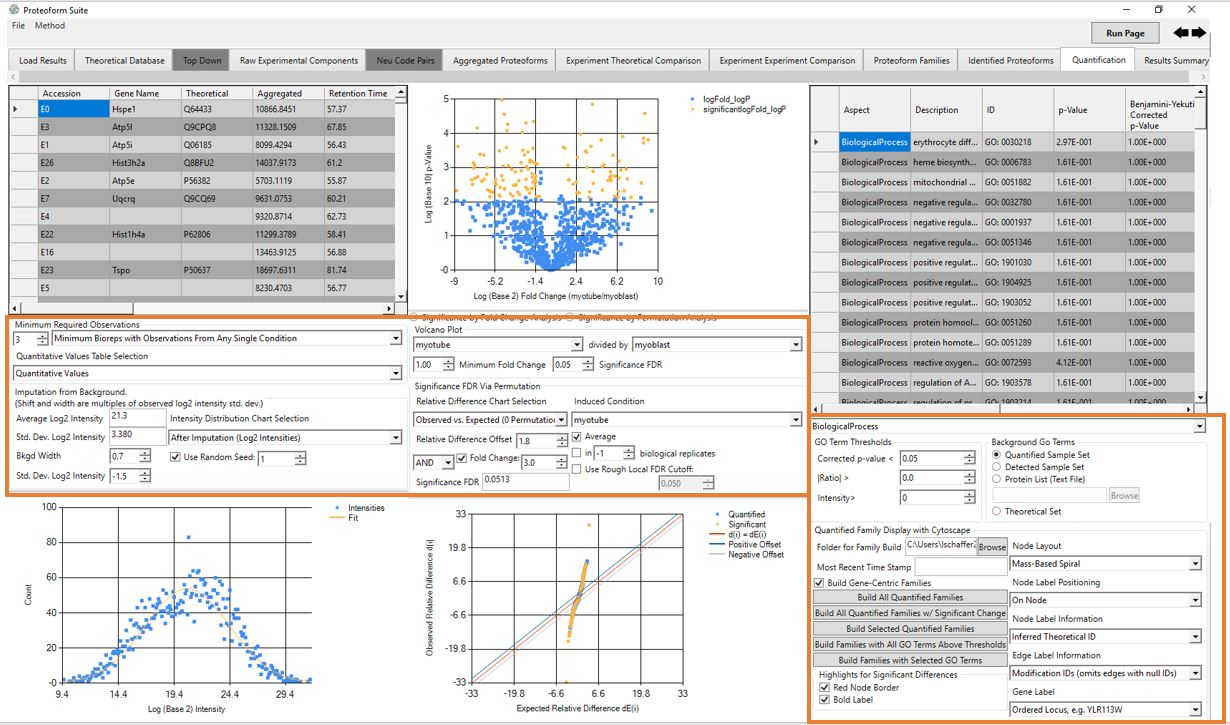
\includegraphics[scale=0.43]{figures/quant1.jpg}
\end{figure}
\begin{itemize}
\item Minimum Required Observations: set the \# (left) and the requirement (right drop down box) to require quantitative observations of an experimental proteoform in more than one file type
\item Quantitative Values Table Selection: select what will be displayed in the Quantitative Values table (top right)
\item Bkgd Width: background distribution for imputation width (sigma)
\item Std. Dev. Log2 Intensity: background distribution for imputation shift, number of sigma from the population mean
\item Use Random Seed: a random seed will be used in the random number generator for selecting imputed intensity values, resulting in the same intensity values each time (with the same given parameters)
\item Significant by Fold Change Analysis: select this option to have the fold change analysis be what determines which experimental proteoforms have statistically significant abundance changes
\item Significance by Perutations: select this option to have the permutation analysis be what determines which experimental proteoforms have statistically significant abundance changes
\item Volcano Plot: choose which condition intensity is divided by which condition intensity
\item Minimum Fold Change: set the minimum log2 fold change for an experimental proteoform's abundance change to be considered significant
\item Significance FDR: set the maximum false discovery rate for an experimental proteoform's abundance change to be considered statistically significant
\item Relative Difference Chart Selection: select which permutation analysis chart is displayed in the bottom middle graph
\item Induced Condition: select which condition is the induced condition
\item Relative Difference Offset: select a minimum relative difference offset from the expected relative difference curve for an abundance change to be considered significant using permutation analysis
\item AND/OR: option to use both relative difference offset and/or a minimum fold change value
\item Fold Change: select a minimum fold change value for an abundance change to be considered significant
\item Average: check this box to use average permutation fold change
\item In \# biological replicates: check this box and set the \# to set a minimum number of biological replicates
\item Use Rough Local FDR cutoff: check this box to use a local false discovery rate cutoff in permutation analysis; set the maximum FDR cutoff below
\item GO Term Dropbox: select which gene ontology terms to display in the Gene Ontology table (top right)
\item GO Term Thresholds: select thresholds for a gene ontology term to be considered significant (maximum p-value, minimum ratio, minimum intensity)
\item Background GO Terms: select what should be used for the background gene ontology terms (quantified only, all detected, or a new protein list loaded in with Browse)
\end{itemize}
\pagebreak
\subsection{Results}
\begin{itemize}
\item Quantitative Values table: this top left table displays quantified experimental proteoforms
\begin{figure}[h]
\centering
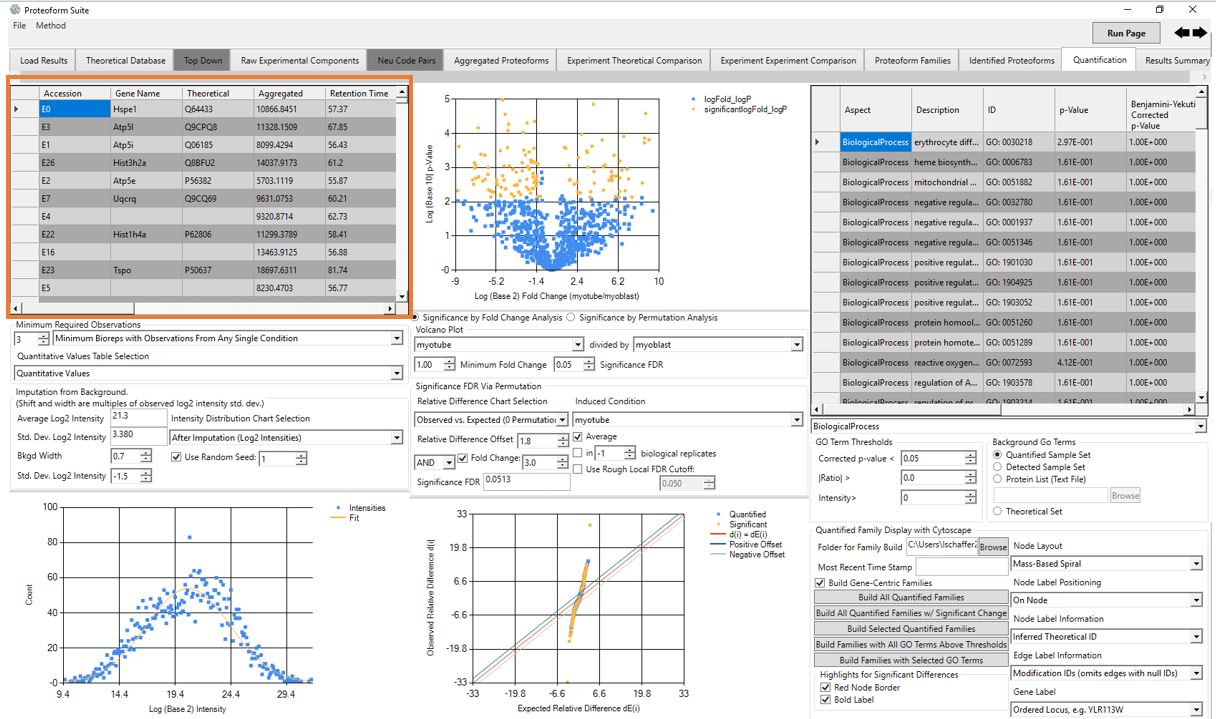
\includegraphics[scale=0.43]{figures/quant2.jpg}
\end{figure}
\begin{itemize}
	\item Accession: unique accession given by Proteoform Suite given to this experimental proteoform
	\item Gene Name: if identified, gene name for this experimental proteoform
	\item Theoretical: if identified, theoretical accession from UniProt for this experimental proteoform
	\item Aggregated Mass: monoisotopic mass of experimental proteoform, weighted average of (light) raw experimental components by intensity
	\item Aggregated RT: retention time of experimental proteoform, average of raw experimental components (unlabeled) or NeuCode pairs (NeuCode labeled)
	\item Condition1 Intensity Sum: summed intensity of raw quantitative components for this condition for this experimental proteoform
	\item Condition2 Intensity Sum: summed intensity of raw quantitative components for this condition for this experimental proteoform
	\item Intensity Sum: total summed intensity of all raw quantitative components (both conditions) for this experimental proteoform
	\item Log2 Fold Change: log2 fold change between 2 conditions for this experimental proteoform
	\item Scatter linear: if significance by permutation analysis, linear intensity
	\item p-value: if significance by fold change analysis, p-value for this experimental proteoform fold change test statistic
	\item Benjamini-Hochberg corrected p-value: if significance by fold change analysis, Benjamini-Hochberg corrected p-value for this experimental proteoform fold change test statistic
	\item Significant: checked if fold change for this experimental proteoform is statistically significant
	\item Student's t-test Statistic: test statistic for log2 fold change analysis t-test
	\item Corresponding Avg. Permuted Student's t-Test Statistic: averaged permuted student's test statistic
	\item Manual Validation: file information for manual validation of most abundant raw quantitative component 
\end{itemize}
\item Imputations from Background: this bottom left graph displays info about the log2 intensities of quantified proteoforms, with an option to view before and after imputation. 
\begin{figure}[h]
\centering
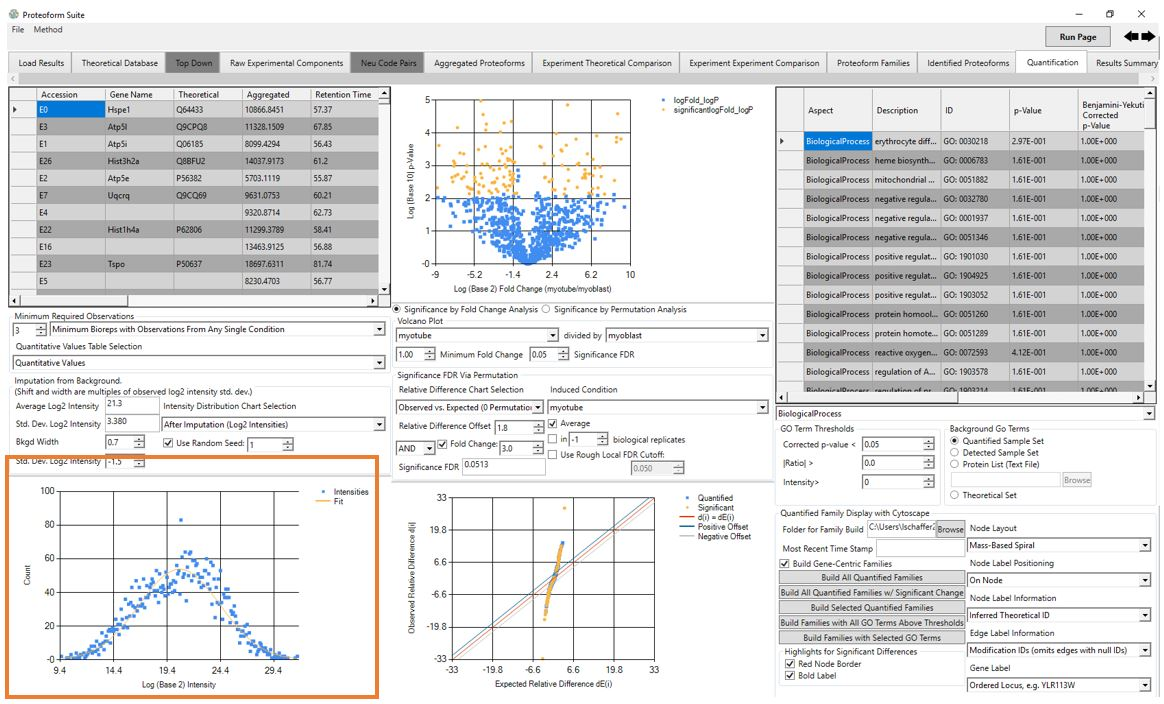
\includegraphics[scale=0.43]{figures/quant3.jpg}
\end{figure}
\pagebreak
\item Volcano plot: this top middle graph shows the a volcano plot from the fold change analysis, p-value vs. log2 fold change. Proteoforms with a statistically significant fold change are yellow, other proteoforms are blue.
\begin{figure}[h]
\centering
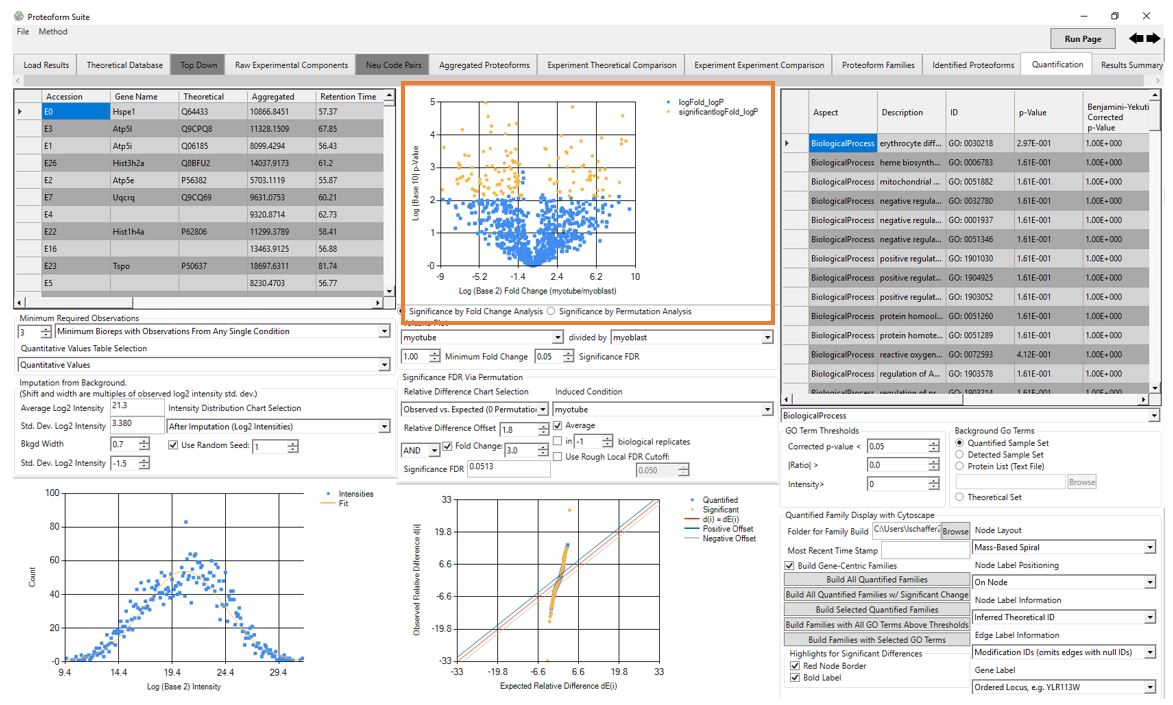
\includegraphics[scale=0.43]{figures/quant4.jpg}
\end{figure}
\item Permutation Analysis graph: the bottom middle graph shows information from the permutation analysis, including observed relative difference vs. expected relative difference
\begin{figure}[h]
\centering
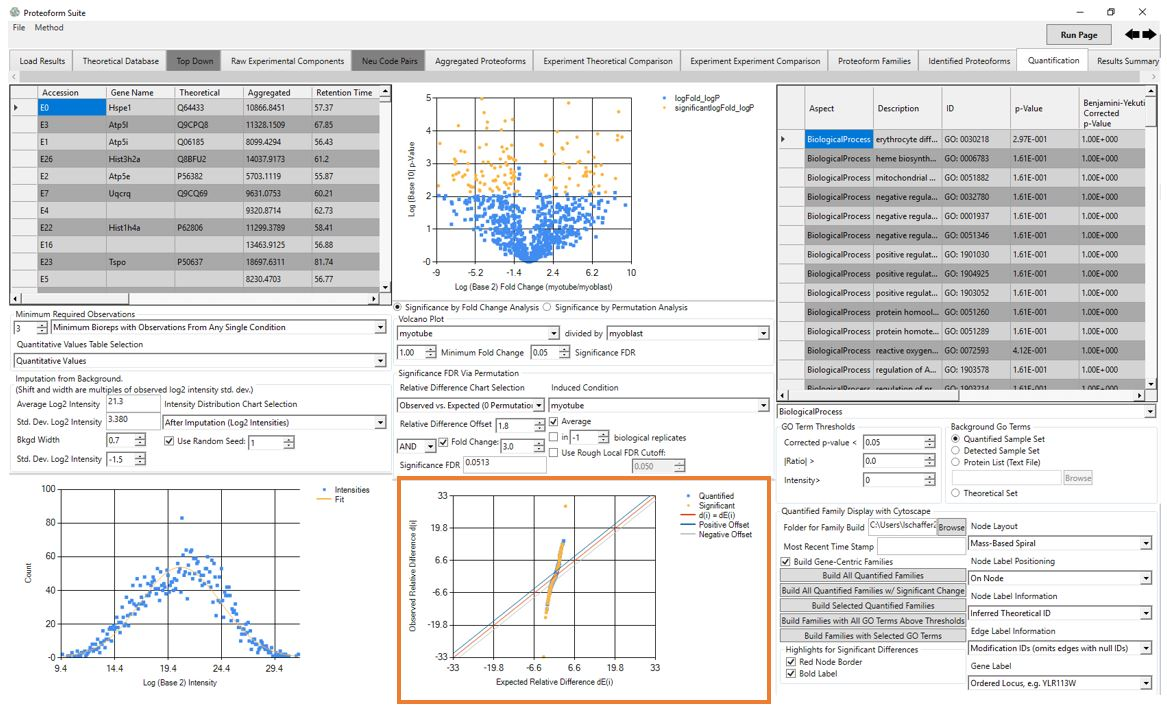
\includegraphics[scale=0.43]{figures/quant5.jpg}
\end{figure}
\item Gene Ontology Terms table: the top right table displays the gene ontology terms
\begin{figure}[h]
\centering
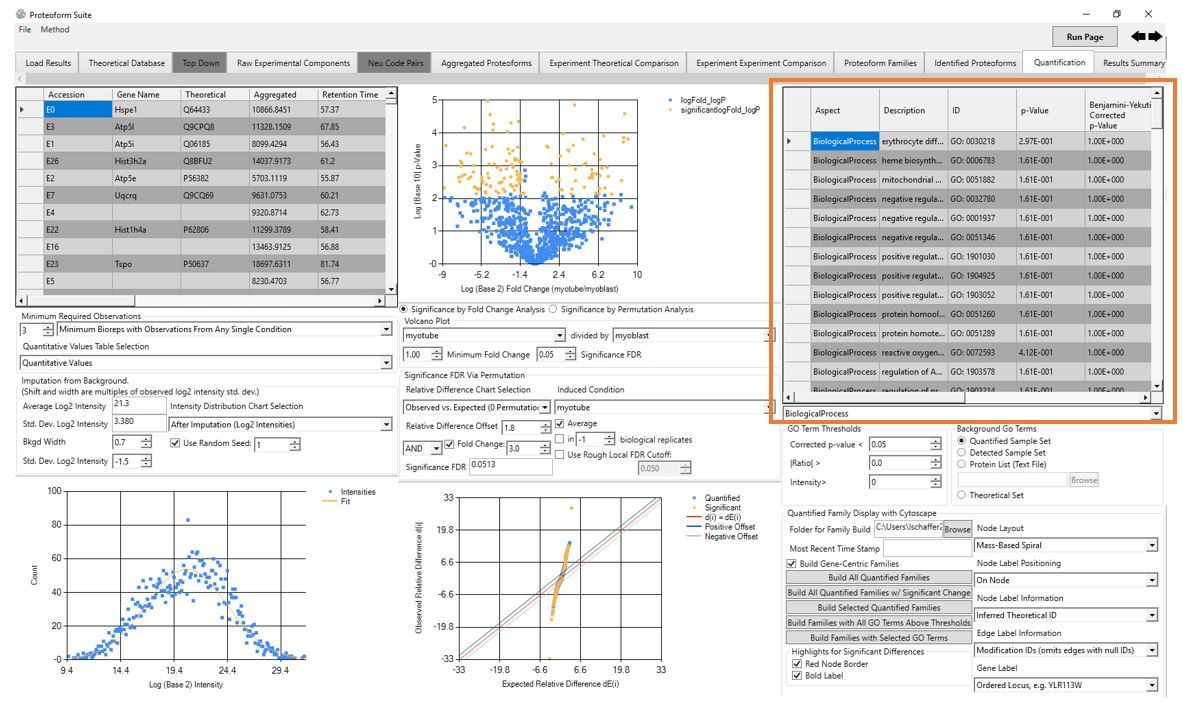
\includegraphics[scale=0.43]{figures/quant6.jpg}
\end{figure}
\begin{itemize}
\item Aspect: gene ontology term type
\item Description: gene ontology term description
\item ID: gene ontology term
\item P-Value: p-value for this gene ontology term
\item Benjamini-Yekutieli Corrected p-Value: Benjamini-Yekutieli corrected p-value for this gene ontology term
\item Log Odds Ratio: log odds ratio
\item Significant Proteins With This Go-Term: number of unique proteins with this GO term and with an experimental proteoform with a statistically significant abundance change
\item Total Significant Proteins: number of unique proteins with an experimental proteoform with a statistically significant abundance change
\item Background Proteins With This Go-Term: number of unique background proteins with this GO term
\item Total Background Proteins: total number of background proteins
\end{itemize}
\item Folder for Family Build: folder to build scripts to visualize proteoform families in Cytoscape
\item Most Recent Time Stamp: time stamp that will be in the filename of scripts to visualize proteoform families in Cytoscape
\item Build Gene-Centric Families: if checked, all proteoforms connected to theoretical proteoforms from the same gene will be grouped into the same proteoform family
\item Build All Quantified Families: exports scripts for Cytoscape to visualize all quantified proteoform families
\item Build All Quantified Families w/ Significant Change: exports scripts for Cytoscape to visualize all quantified proteoform families with at least one experimental proteoform with a statistically significant abundance change
\item Build Selected Quantified Families: exports scripts for Cytsocape to visualize proteoform families with an experimental proteoform selected in the Quantification Values table
\item Build Families with All GO Terms Above Threshold: exports scripts for Cytoscape to visualize all quantified proteoform families with gene ontology terms above threshold
\item Build Families with Selected GO Terms: exports scripts for Cytoscape to visualize proteoform families with a gene ontology term selected in the Gene Ontology Terms table
\item Highlights for Significant Differences: if checked, a red node border and bold label will be used in quantitative proteoform families to highlight experimental proteoforms with statistically significant quantitative differences
\item Node Layout: this drop-down box changes the node layout in visualized proteoform families in Cytoscape
\item Node Label Positioning: this drop-down box changes the position of node labels in visualized proteoform families in Cytoscape
\item Node Label Informing: this drop-down box changes the node label information in visualized proteoform families in Cytoscape
\item Edge Label Information: this drop-down box changes the edge label information in visualized proteoform families in Cytoscape
\item Preferred Gene Label: this drop-down box changes the gene label information in visualized proteoform families in Cytoscape
\end{itemize}